\documentclass[12pt,fleqn]{article}\usepackage{../../common}
\begin{document}
Sezonsallık, Trend Çıkartmak, Değişim Noktası, CUSUM

\begin{minted}[fontsize=\footnotesize]{python}
def model_compute(X, coef):
   degree = len(coef)-1
   curve = [np.sum([coef[-1]] + [x**(degree-d)*c for d,c \
            in enumerate(coef[:-1])]) for x in X]
   return curve
\end{minted}


\begin{minted}[fontsize=\footnotesize]{python}
from pandas import datetime
def parser(x):
    return datetime.strptime( '190'+x, '%Y-%m' )
    
df = pd.read_csv('shampoo-sales.csv', header=0, index_col=0, \
     parse_dates=True, date_parser=parser)

X = np.array(range(len(df))).reshape(-1)
y = df.values.reshape(-1)
degree = 1
coef = np.polyfit(X, y, degree)
df['Model']  = model_compute(X, coef)
df.plot()
plt.savefig('tser_022_de_01.png')
\end{minted}

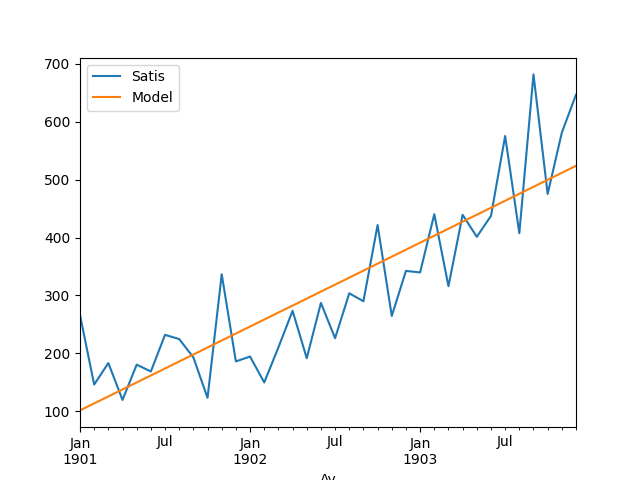
\includegraphics[height=6cm]{tser_022_de_01.png}


\begin{minted}[fontsize=\footnotesize]{python}
detrended = df.Satis-df.Model
detrended.plot()
plt.savefig('tser_022_de_03.png')
\end{minted}

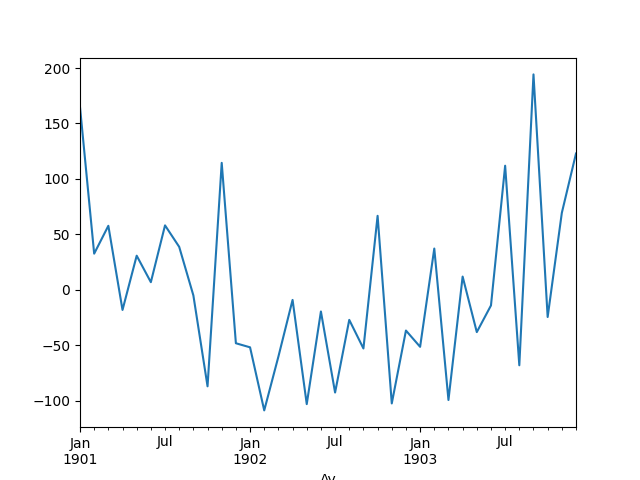
\includegraphics[height=6cm]{tser_022_de_03.png}



\begin{minted}[fontsize=\footnotesize]{python}
import pandas as pd
df = pd.read_csv('daily-min-temperatures.csv', header=0,\
                 index_col=0, parse_dates=True)
X = [i%365 for i in range(0, len(df))]
y = df.values
degree = 4
coef = np.polyfit(X, y, degree)
df['Model']  = model_compute(X, coef)
df.plot()
plt.savefig('tser_022_de_02.png')
\end{minted}


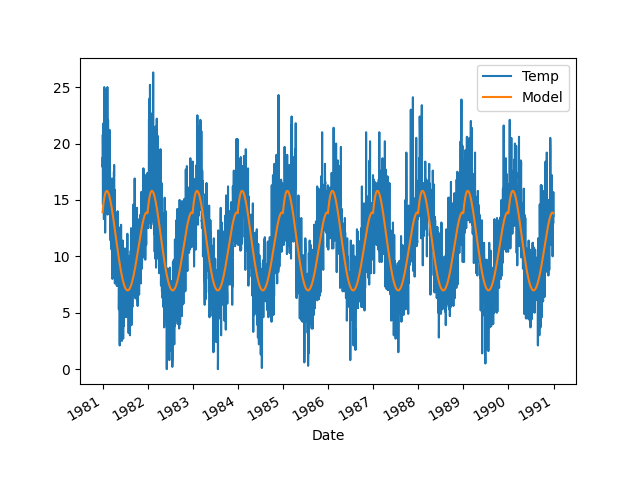
\includegraphics[height=6cm]{tser_022_de_02.png}

\begin{minted}[fontsize=\footnotesize]{python}
detrended = df.Temp-df.Model
detrended.plot()
plt.savefig('tser_022_de_04.png')
\end{minted}


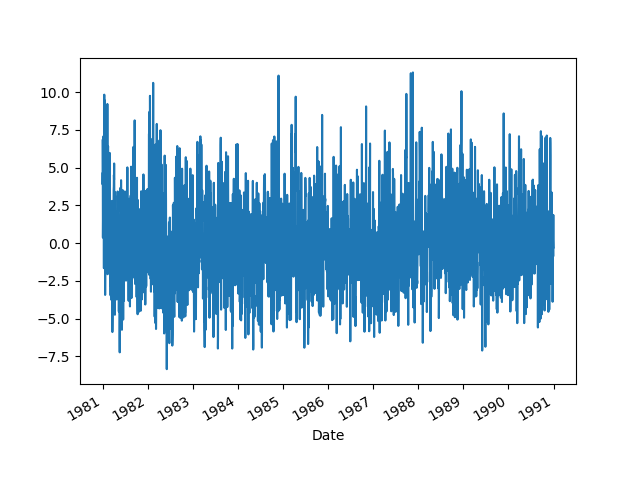
\includegraphics[height=6cm]{tser_022_de_04.png}



Cusum

\inputminted[fontsize=\footnotesize]{python}{cusum.py}

\begin{minted}[fontsize=\footnotesize]{python}
import pandas as pd
  
y = np.random.randn(300)/5
y[100:200] += np.arange(0, 4, 4/100)
x = range(len(y))
df = pd.DataFrame(y,columns=['y'])
df['x'] = x
df = df.set_index('x')
df.y.plot()
plt.savefig('tser_022_de_05.png')
\end{minted}

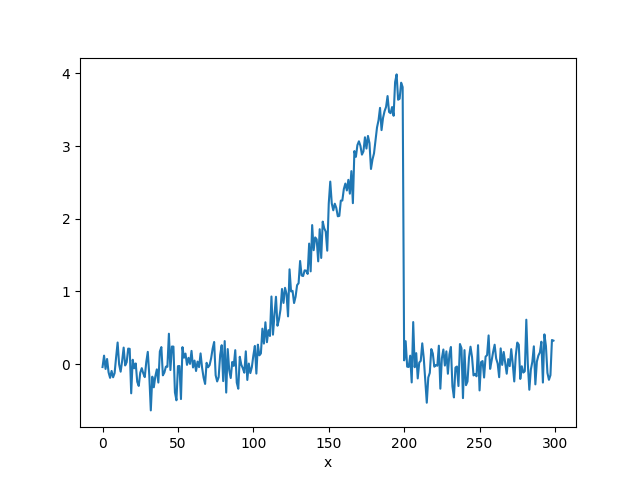
\includegraphics[height=6cm]{tser_022_de_05.png}

\begin{minted}[fontsize=\footnotesize]{python}
import cusum
ta, tai, taf, amp = cusum.detect_cusum(df.y, 2, .02, True, True)

fig, ax = plt.subplots(1, 1)
t = range(df.y.size)
ax.plot(t, df.y, 'b-', lw=2)
if len(ta):
    ax.plot(tai, df.y[tai], '>', mfc='g', mec='g', ms=10, label='Start')
    ax.plot(taf, df.y[taf], '<', mfc='g', mec='g', ms=10, label='Ending')
    ax.plot(ta, df.y[ta], 'o', mfc='r', mec='r', mew=1, ms=5, label='Alarm')
    
plt.savefig('tser_022_de_06.png')
\end{minted}

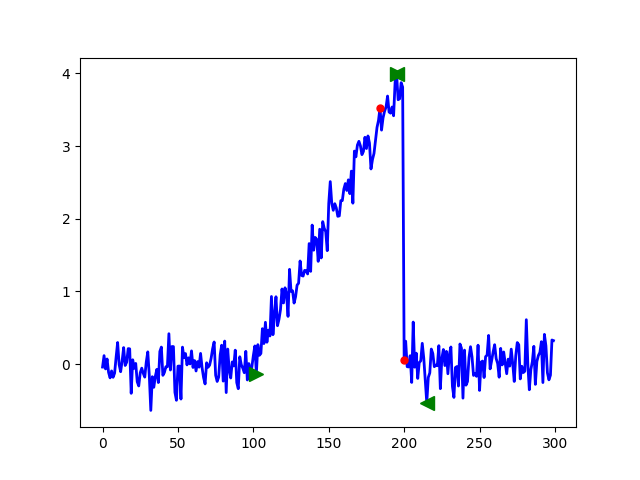
\includegraphics[height=6cm]{tser_022_de_06.png}

\begin{minted}[fontsize=\footnotesize]{python}
print (len(ta))
print ('Baslangic =', tai[0], 'Bitis =', taf[0])
\end{minted}

\begin{verbatim}
2
Baslangic = 95 Bitis = 197
\end{verbatim}




 












Kaynaklar

[1] Brownlee, {\em Introduction to Time Series Modeling with Python}

[2] Github, \url{https://raw.githubusercontent.com/BMClab/BMC/master/functions/detect_cusum.py}

[3] MIT, {\em OCW Single Variable Calculus, unit 5, Session 99},
         \url{https://ocw.mit.edu/courses/mathematics/18-01sc-single-variable-calculus-fall-2010/index.htm}

\end{document}
